\chapter{Mock-up}
A seguito dei problemi di usabilità evidenziati nei capitoli precedenti, siamo passati alla fase di stesura di possibili soluzioni. L'elaborazione di modelli, grafici che mirano a risolvere i problemi riscontrati, o che quantomeno ne riducano drasticamente la criticità, prendono il nome di mock-up.\\
\'E da sottolineare come i mock-up siano un'astrazione e spesso siano un compromesso atto a  migliorare l'usabilità del sito web in esame; la scelta di tale compromesso è influenzata dalle conoscenze del gruppo e dalle rispettive esperienze pregresse.\\
Prima di intervenire abbiamo stabilito l'approccio col quale affrontare i problemi:
\begin{itemize}
\item Singolarmente: ha il vantaggio di trattare modularmente ogni problema e ridurre cos il rischio di generare nuovi problemi, durante la risoluzione. Lo svantaggio maggiore  rappresentato dal fatto che con questo metodo si rischia di generare ridondanza e di creare confusione per l'utente.
\item Per gruppi o collezioni:  l'opposto del caso precedente. Si riduce la ridondanza, mirando a ottenere una visone più ampia dei problemi per trovare  soluzioni che possano andare bene per pi problemi contemporaneamente. In questo modo invece aumenta il rischio di generare nuovi problemi.
\end{itemize}
Nel nostro caso  stata scelta la seconda tecnica, in quanto trattandosi spesso di gruppi di pagine, era preferibile avere una visione d'insieme e trattare errori trasversali a pi pagine, piuttosto che concentrarsi su errori di visibilit limitata.\\
C'è anche un altro aspetto da mettere in evidenza, che spesso viene trascurato: il mock-up, inteso come strumento di presentazione solamente grafico, pertanto si potranno avere solo degli screenshot di quello che potrebbe essere il risultato, nel caso la modifica riguardi il layout della pagina, ma come si è spesso notato, alcuni degli errori più gravi, riguardano l'aspetto implementativo; su tali errori si può solamente ragionare a livello teorico, ma l'implementazione di una soluzione non è fattibile in quanto mancano gli strumenti necessari alla realizzazione.\\ 
Verrà poi ricordato che nelle varie sottosezioni, spesso vengono proposte soluzioni, che andrebbero replicate su molte pagine del sistema. In genere si tratta di link dai nomi non chiari, o la mancanza di collegamenti che, se inseriti nel posto corretto, migliorerebbero l'usabilità.\\
\newline
Per poter iniziare la concettualizzazione dei mock-up è stato necessario lavorare in due fasi:
\begin{itemize}
\item Durante la prima fase abbiamo lavorato direttamente sul codice HTML e sui fogli di stile, i cosiddetti CSS. Per modificarli abbiamo impiegato FireBug, un debugger JavaScript, che, tra le altre cose, permette di modificare "a caldo" il codice interpretato dal browser, vedendo immediatamente risultati delle modifiche. Inoltre l'uso di FireBug ci ha permesso di inserire nuovi link e nuovo testo, col medesimo stile del sito Dell. Più nel dettaglio i font utilizzati, i colori di sfondo e altri aspetti legati ai CSS sono rimasti invariati, avendo un riscontro immediato della pagina mostrata all'utente.
\item Durante la seconda fase invece abbiamo impiegato programmi di grafica (Gimp, Paint, Photoshop), utilizzandoli per i ritocchi più pesanti apportati alle pagine. Sono stati utilizzati prevalentemente, quando la modifica del codice avrebbe richesto troppo tempo. Ad esempio per posizionare immagini e blocchi di testo in determinate posizioni all'interno della pagina, o creare riquadri con gli angoli smussati, che in HTML avrebbero richiesto uno sforzo eccessivo. in tal modo, tramite ``taglia e incolla'' abbiamo potuto disporre rapidamente gli elementi nella maniera che si è ritenuta più oppurtuna
\end{itemize}
\section{Mock-up home page sezione casa}
Prima di procedere con la presentazione dei mock-up ideati per questa sezione vi � un concetto che � bene ricordare: alcuni dei cambiamenti illustrati in questa sezione andrebbero riportati su tutte le pagine del sito web, poich� il problema di usabilit� evidenziato � talvolta presente su tutte le pagine del sito web, in questi casi verr� esplicitamente .\\
\begin{figure}[!h]
\centering
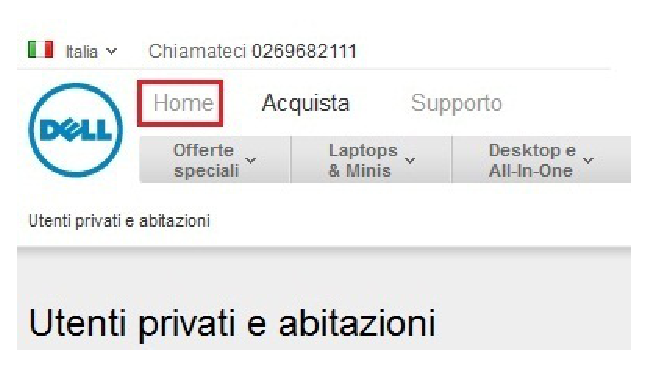
\includegraphics[scale=0.8]{figure/mock_up_home_page.eps}
\caption{Evidenziato in rosso il nuovo link all'Home page. Questo mock-up si applica a tutte le pagine del sito.}
\label{fig:mock_up_non_loggato}
\end{figure}
\begin{figure}[!h]
\centering
\includegraphics[scale=0.8]{figure/mock_up_home_page2.eps}
\caption{Evidenziato in rosso il nuovo link all'Home page. Questo mock-up si applica a tutte le pagine del sito.}
\label{fig:mock_up_non_loggato2}
\end{figure}
\begin{figure}[!h]
\centering
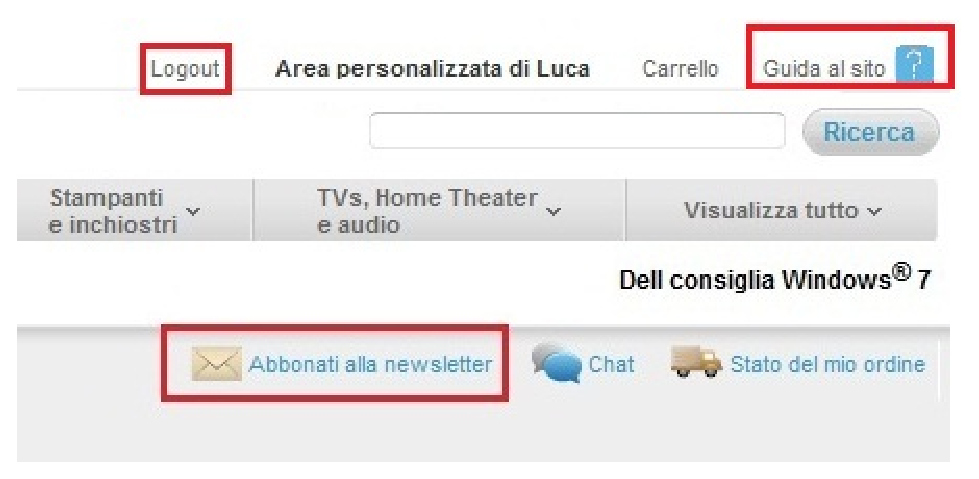
\includegraphics[scale=0.8]{figure/mock_up_home_page_loggato.eps}
\caption{Evidenziate in rosso le modifiche apportate alla home page quando l'utente � loggato.}
\label{fig:mock_up_loggato}
\end{figure}
{\bf Descrizione:} non � immediatamente visibile un link per il ritorno all'home page, non c'� un link diretto che permetta a un nuovo utente di registrarsi e infine il link che punta alla guida al sito � posto in fondo alla pagina, nascosto tra altri link e senza essere posto in evidenza in alcun modo. Il link ``Registrazione e-mail'' non fornisce sufficienti informazioni sull'effetto di tale registrazione.\\
{\bf Proposta di soluzione:} le soluzioni introdotte sono mostrate nelle figure \ref{fig:mock_up_non_loggato} e \ref{fig:mock_up_non_loggato2}. Pi� nel dettaglio abbiamo aggiunto un link ``Home'' sotto al logo Dell, che punta all'home page. La idea di metterlo sotto � stata concepita per separarlo spazialmente dai due link che portano alla sezione per gli acquisti e per il supporto, per marcare ulteriormente questa differenza � stato inoltre impiegato il medesimo colore del logo Dell.\\
A destra del logo sono posizionati due link: ``Registrati'' e ``Guida al sito'', i quali sono stati incorniciati in due linguette, ispirandoci all'idea delle cosiddette tab utilizzate nei moderni web browser (in Firefox e in Chrome, per citarne alcuni). Ci� serve a dare un'idea intuitiva che ci siano due sezioni separate, ma immediatamente accessibili tramite queste linguette. Per completare il mock-up che fa riferimente alla pagina visualizzata quando l'utente non � ancora loggato (figura: \ref{fig:mock_up_non_loggato2}) abbiamo anche pensato di modificare la dicitura ``Sign In'' con ``Accedi''. Nella parte sottostante il link ``Registrazione e-mail'' � stato sostituito con ``Abbonati alla newsletter'', con l'intento di fugare ogni dubbio riguardo allo scopo della sottoscrizione.\\
Per quanto riguarda i link che fanno riferimento alla pagina personale e al logout, abbiamo pensato di rimuovere la parte tra parentesi della dicitura ``Area personalizzata di Luca (L'utente corrente non � Luca?)'', ritenuta ridondante, e affiancarla da un opportuno link di logout.\\
\newline
In questa sezione abbiamo deciso d'inserire anche il mock-up del form di login, modificato come in figura \ref{fig:form_login}.\\
{\bf Descrizione:} Il form del login � di per s� molto semplice e non ha avuto bisogno di un restyling degno di nota. Ci� che rappresenta il problema fondamentale, � il corretto funzionamento del sistema a fronte di due casi:
\begin{itemize}
\item Se si chiude la finestra di login durante la visualizzazione della progress bar, e successivamente si richiede un nuovo login il sitema � ancora in attesa della verifica dei dati inseriti precedentemente. A questo punto viene mostrata una pagina che riporta "caricamento in corso", tuttavia lo stato del sistema non cambia fintanto che l'utente non carica un'altra pagina o non effettua il refresh della pagina corrente.
\item Dopo sei tentativi errati d'inserimento delle credenziali il sistema dovrebbe procedere alla disattivazione dell'account. Tuttavia inserendo le credenziali corrette, anche dopo sei tentativi errati l'account continua a funzionare.
\end{itemize} 
{\bf Proposta di soluzione:} come accennato in precedenza l'aspetto grafico della finestra non necessita di grossi cambiamenti, e l'unico ad essere introdotto � una label che spiega il significato degli asterischi.\\ 
Diverso � l'intervento implementabile:
\begin{itemize}
\item Durante la fase di autenticazione, mentre � mostrata la progress bar, se la finestra viene chiusa, il sistema dovrebbe cercare di ritornare allo stato precedente a quello dell'inserimento dei dati, nel caso il browser non reindirizzasse l'utente � invtato a cliccare su un apposito link (descrizione e mock-up pi� avanti AAAAAAAAAAAAAAAAAAAAAAAAAAAAAAAAAAAAAAAAAAAAAAAAAAAAAAAAAAA\\AAAAAAAAAAAAAAAAAAAAAAAAAAAAAAAAAAAAAAAAAAAAAAAAAAAAA sarebbe meglio dare un riferimento). 
\item Per quanto riguarda la disattivazine dell'account abbiamo invece pensato che che sarebbe pi� opportuno disattivare temporaneamente la possibilit� di login dall'indirizzo ip dal quale sono provenuti i tentativi di login falliti. Questo per prevenire che utenti malintenzionati falliscano intenzionalmente il login per bloccare l'account. Il nostro approccio limiterebbe comunque la portata di attacchi di tipo brute-force.\\ 
\end{itemize}
\begin{figure}[!h]
\centering
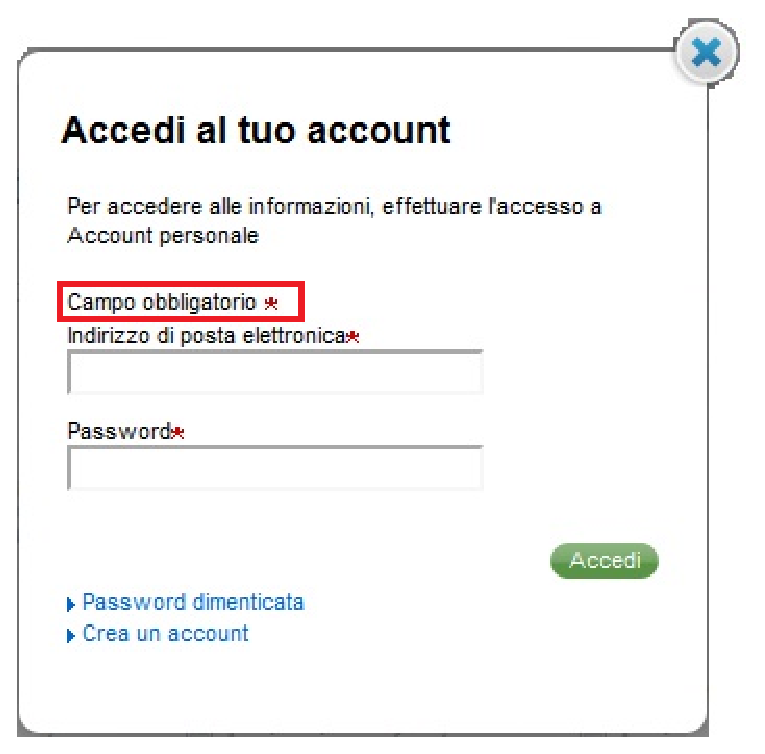
\includegraphics[scale=0.65]{figure/mock_up_fom_login.eps}
\caption{Evidenziate in rosso le modifiche apportate alla home page quando l'utente � loggato}
\label{fig:form_login}
\end{figure}

{\bf Descrizione}: all'interno della pagina relativa ai dati personali dell'utente non esiste un link che rimandi alla pagina in cui l'utente pu� cancellare il proprio account. Ci� pu� essere vincolante poich�, a nostro avviso, un utente dovrebbe avere la libert� di potersi ritirare la propria iscrizione in ogni momento.
{\bf Proposta di soluzione}: all'interno della pagina contenente i dati personali viene aggiunta una voce al men� di sinistra chiamata ``cancellazione account''. In tal modo si pu� accedere a una sezione, che verr� aperta sulla destra rispetto al men�, in cui l'utente potr� cancellare il proprio account. Dal punto di vista implementativo, si � pensato che fosse opportuno far comparire un popup che chieda l'inserimento della password dell'utente per confermare la cancellazione,come vincolo di sicurezza contro cancellazioni accidentali.(figura \ref{fig:mockup_cancellazione_account}).

\begin{figure}[!h]
\centering
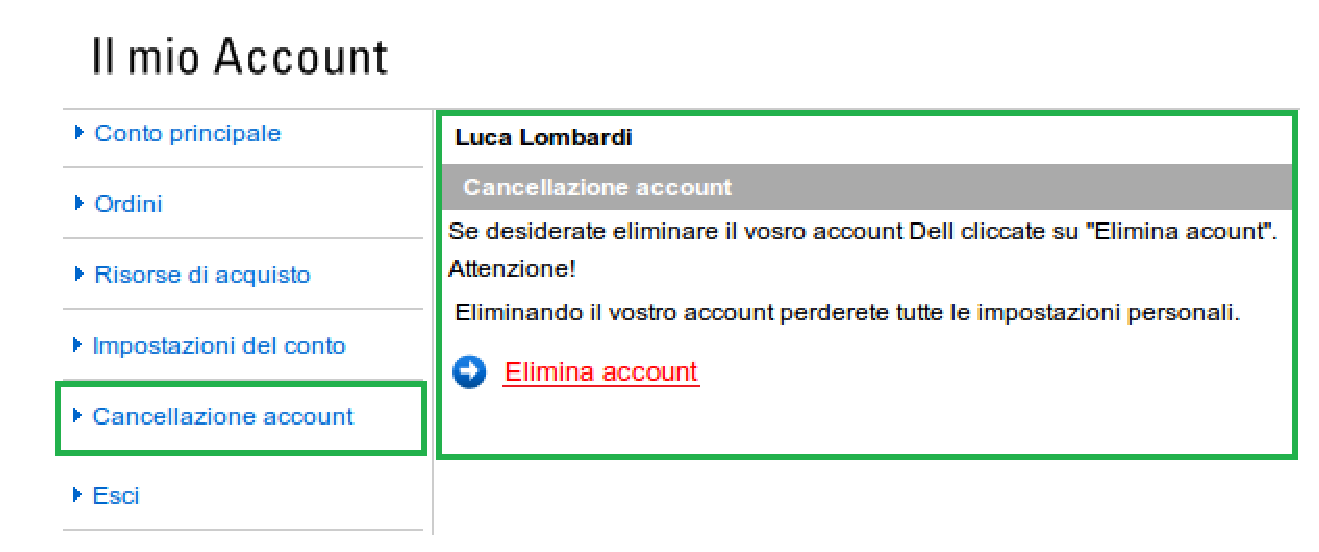
\includegraphics[scale=0.7]{figure/mock_up_cancellazione.eps}
\caption{In verde sono evidenziate le parti aggiunte che consentono all'utente di cancellare il proprio account.}
\label{fig:mockup_cancellazione_account}
\end{figure}

{\bf Descrizione}: come anticipato nella sezione dedicata ai problemi di usabilit�, se l'utente chiude la finestra di dialogo, nel momento in cui il sistema sta verificando le credenziali, il sitema rimane in uno stato ibrido in cui l'utente non pu� effettuare un nuovo login e il sistema non riconosce ancora l'utente.\\
{\bf Proposte di soluzione}: per ovviare a tale problema abbiamo pensato di introdurre una redirezione automatica dalla pagina che compare alla chiusura della finestra di dialogo, nel caso in cui il browser fallisse la redirezione diamo all'utente la possibilit� di forzare il sistema ad uscire dallo stato nel quale � caduto. Mock-up mostrato in figura \ref{fig:mock_up_login_reindirizzo}. \\

\begin{figure}[!h]
\centering
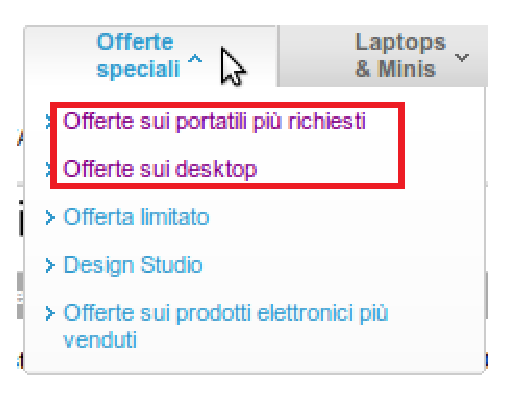
\includegraphics[scale=0.6]{figure/mock_up_link_usati.eps}
\caption{Riquadrati in rosso la modfica del colo dei link gi� selezionati dall'utente}
\label{fig:mock_up_link_usati}
\end{figure}

{\bf Descrizione}: come segnalato in precedenza, il sistema spesso non offre all'utente un riscontro sui link gi� usati (per esempio nei menu a tendina in cima alla pagina), all'interno di una stessa sessione di lavoro.\\
{\bf Proposte di soluzione}: come riportato in figura \ref{fig:mock_up_link_usati} si pu� notare come i link selezionati almeno una volta siano colorati in modo diverso, dando all'utente un aiuto qualora cerchi una pagina visitata in precedenza e l'operatore di BACK del browser non gli possa essere d'aiuto.

\begin{figure}[!h]
\centering
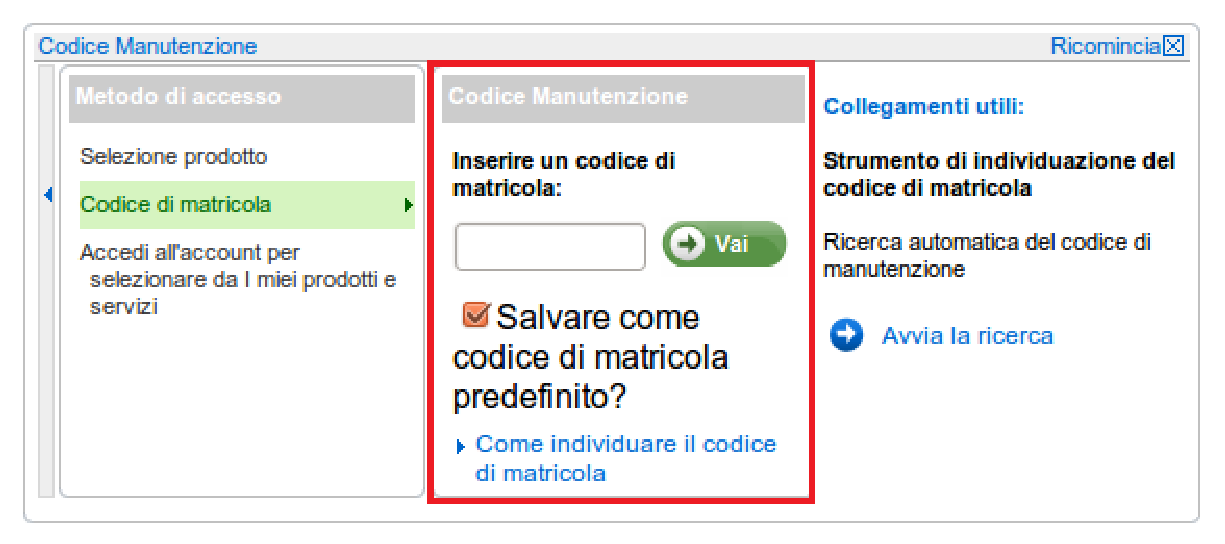
\includegraphics[scale=0.75]{figure/mock_up_manutenzione.eps}
\caption{il men� viene espanso leggermente per evitare la scroll bar, come invece era fatto nella versione originale (figura:\ref{fig:manutenzione})}
\label{fig:mock_up_manutenzione}
\end{figure}

{\bf Descrizione}: dalla figura \ref{fig:manutenzione} si pu� vedere che l'area dedicata al ``Codice di matricola'', � estramente ridotta e si deve ricorrere a una scroll bar per consentire all'utente di visualizzare tutto il contenuto: abbiamo in questo caso un help nascosto, ci� risulta estremamente scomodo, considerato che nella pagina � presente molto spazio inutilizzato.\\
{\bf Proposte di soluzioni}: viene ampliata l'intera area, fino a che la scroll bar non scompare, in tal modo l'utente pu� accedere a tutte le informazioni in modo diretto.


\begin{figure}[!h]
\centering
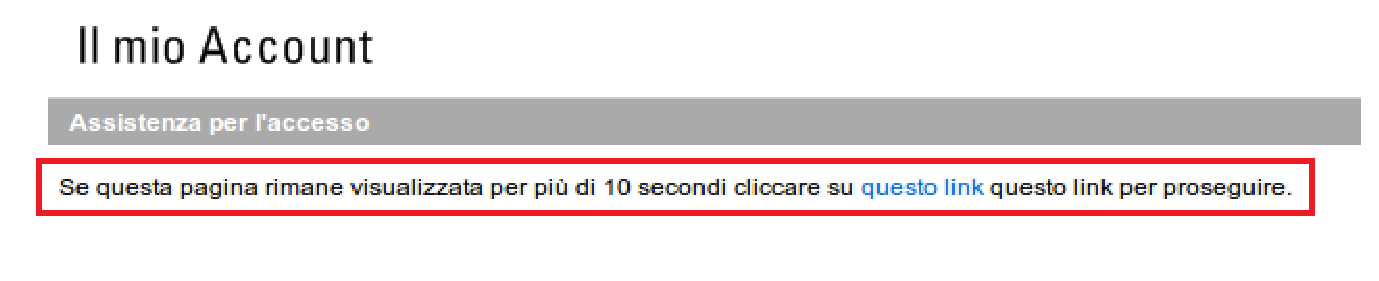
\includegraphics[scale=0.6]{figure/mock_up_login_reindirizzo.eps}
\caption{Nel caso il form del login non reindirizzi automaticamente, viene data la possibilit� all'utente di agire manualmente}
\label{fig:mock_up_login_reindirizzo}
\end{figure}
{\bf Descrizione}: nella figura \ref{fig:mock_up_riepilogo} sono evidenziate le modifiche apportate alla pagina di configurazione del propriro sistema Dell. Come anticipato nella sezione relativa ai problemi di usabilit�, la pagina relativa alla scelta per la copertura sui danni accidentali, non ha alcun riferimento alle condizioni contrattuali, ma solo vaghe spiegazioni dal carattere pubblicitario. Inoltre la finestra di riepilogo delle componenti scelte per la personalizzazione � molto ristretta, costringendo l'utente a un continuo uso dello scroll per scorrere tale riassunto.\\
{\bf Proposta di soluzione}: viene aggiunto un link alla documentazione per gli esatti termini contrattuali dell'estensione di garanzia proposta. Inoltre la finestra di riepilogo dei componenti selezionati dall'utente, posta nella parte destra della pagina, viene espansa in modo da mostrare pi� componenti contemporaneamente.
\begin{figure}[!h]
\centering
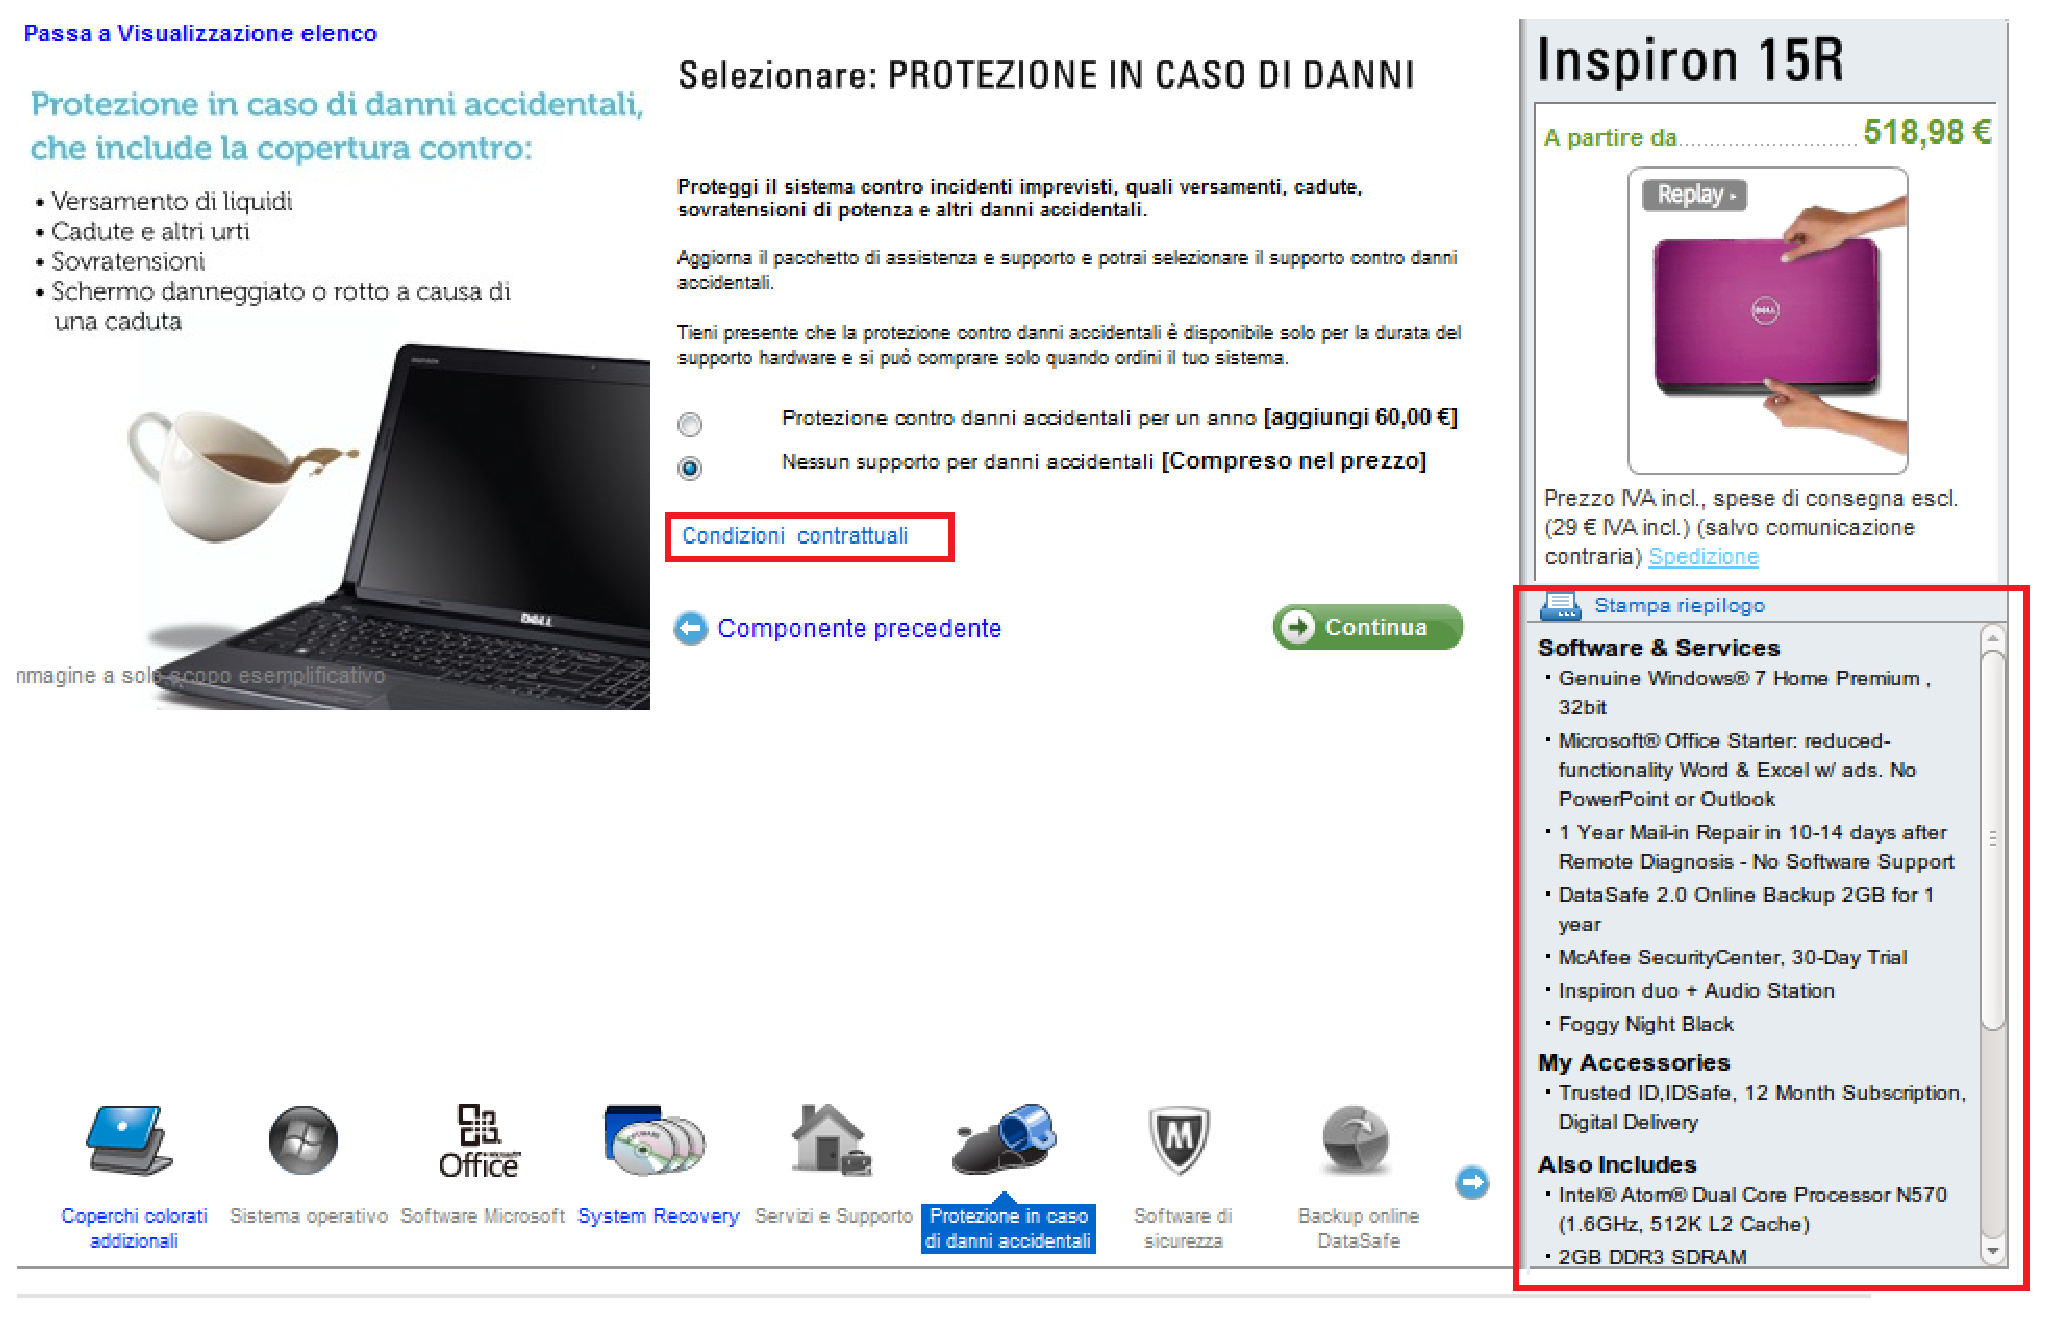
\includegraphics[scale=0.7,angle=90]{figure/mock_up_riepilogo.eps}
\caption{Mock-up sulla pagina di configurazione del computer}
\label{fig:mock_up_riepilogo}
\end{figure}
\newline
{\bf Descrizione}: come anticipato nella sezione relativa ai problemi di usabilit�, un problema di un certo rilievo � il sovraffollamento delle due sezioni ``Acquista'' e ``Supporto'', che rendono difficoltosa la navigazione. 
Di seguito analizzeremo le due soluzioni proposte, motivando le scelte effettuate.
\begin{itemize}
\item {\bf Sezione Acquisti}: innanzitutto � stata analizzata la home page della sezione degli acquisti. Come si pu� notare dalle figura mostrata nella sezione relativa ai problemi di usabilit�, in figura \ref{fig:schermata_incasinata}, la pagina mostrata all'utente � troppo densa densa di informazioni, i titoli delle macrosezioni non sono cliccabili, sono presenti link duplicati che puntano alle medesime sezioni e al tutto sono mescolati banner pubblicitari. Sicuramente � utile usare banner pubblicitari per mettere in risalto alcuni prodotti, siccome il sito ha anche lo scopo di essere una vetrina d'esposizione per i propri prodotti, tuttavia la loro collocazione spaziale inficia la navigabilit�.\\

{\bf Proposte di soluzione}: per ovviare a tali problemi si � pensato a una totale riorganizzazione e razionalizzazione dei contenuti, senza la contempo precludere la possibilit� di aggiungere della pubblicit�. \\
Nella figura \ref{fig:mockup_sez_acquisti_pagina_intera} si pu� vedere come si � pensato di riorganizzare il tutto:
\begin{itemize}
Di seguito elenchiamo i cambiamenti introdotti dal mock-up:
\item Innanzitutto spariscono tutte le immagini pubblicitarie che, eventualmente, potranno essere poste ai lati del corpo centrale della pagina.
\item Delle sei sezioni presenti in precedenza (vedere figura:\ref{fig:schermata_incasinata}) ne manteniamo solo quattro, scelte in modo tale che racchiudano tutti i prodotti: ``Notebook \& Mini'', ``Desktop e All-in-One'', ``Monitor'', ``Elettronica e Accessori''. Tramite esse si accede alle varie sottosezioni. Si � ritenuto utile porre al di sotto di ogni immagine alcuni link, come acceleratori per accedere direttamente alle pagine relative alle principali sotto-categorie. In ogni caso abbiamo cercato di fare si che tali link non costituiscono la parte preponderante della pagina e non siano d'intralcio durante la navigazione.
\item Al di sotto di questa sezione vengono proposte due sezioni in chiara evidenza, nel caso l'utente necessitasse di assistenta per l'acquisto di un prodotto. Le due aree scelte sono dedicate all'assistenza tramite chat, oppure assistenza telefonica. L'assistenza tramite chat rimanda all'apposita sezione, all'assistenza telefonica invece non ne � dedicata nessuna, riportando solo il numero di telefono.  
\end{itemize}

\begin{figure}[!h]
\centering
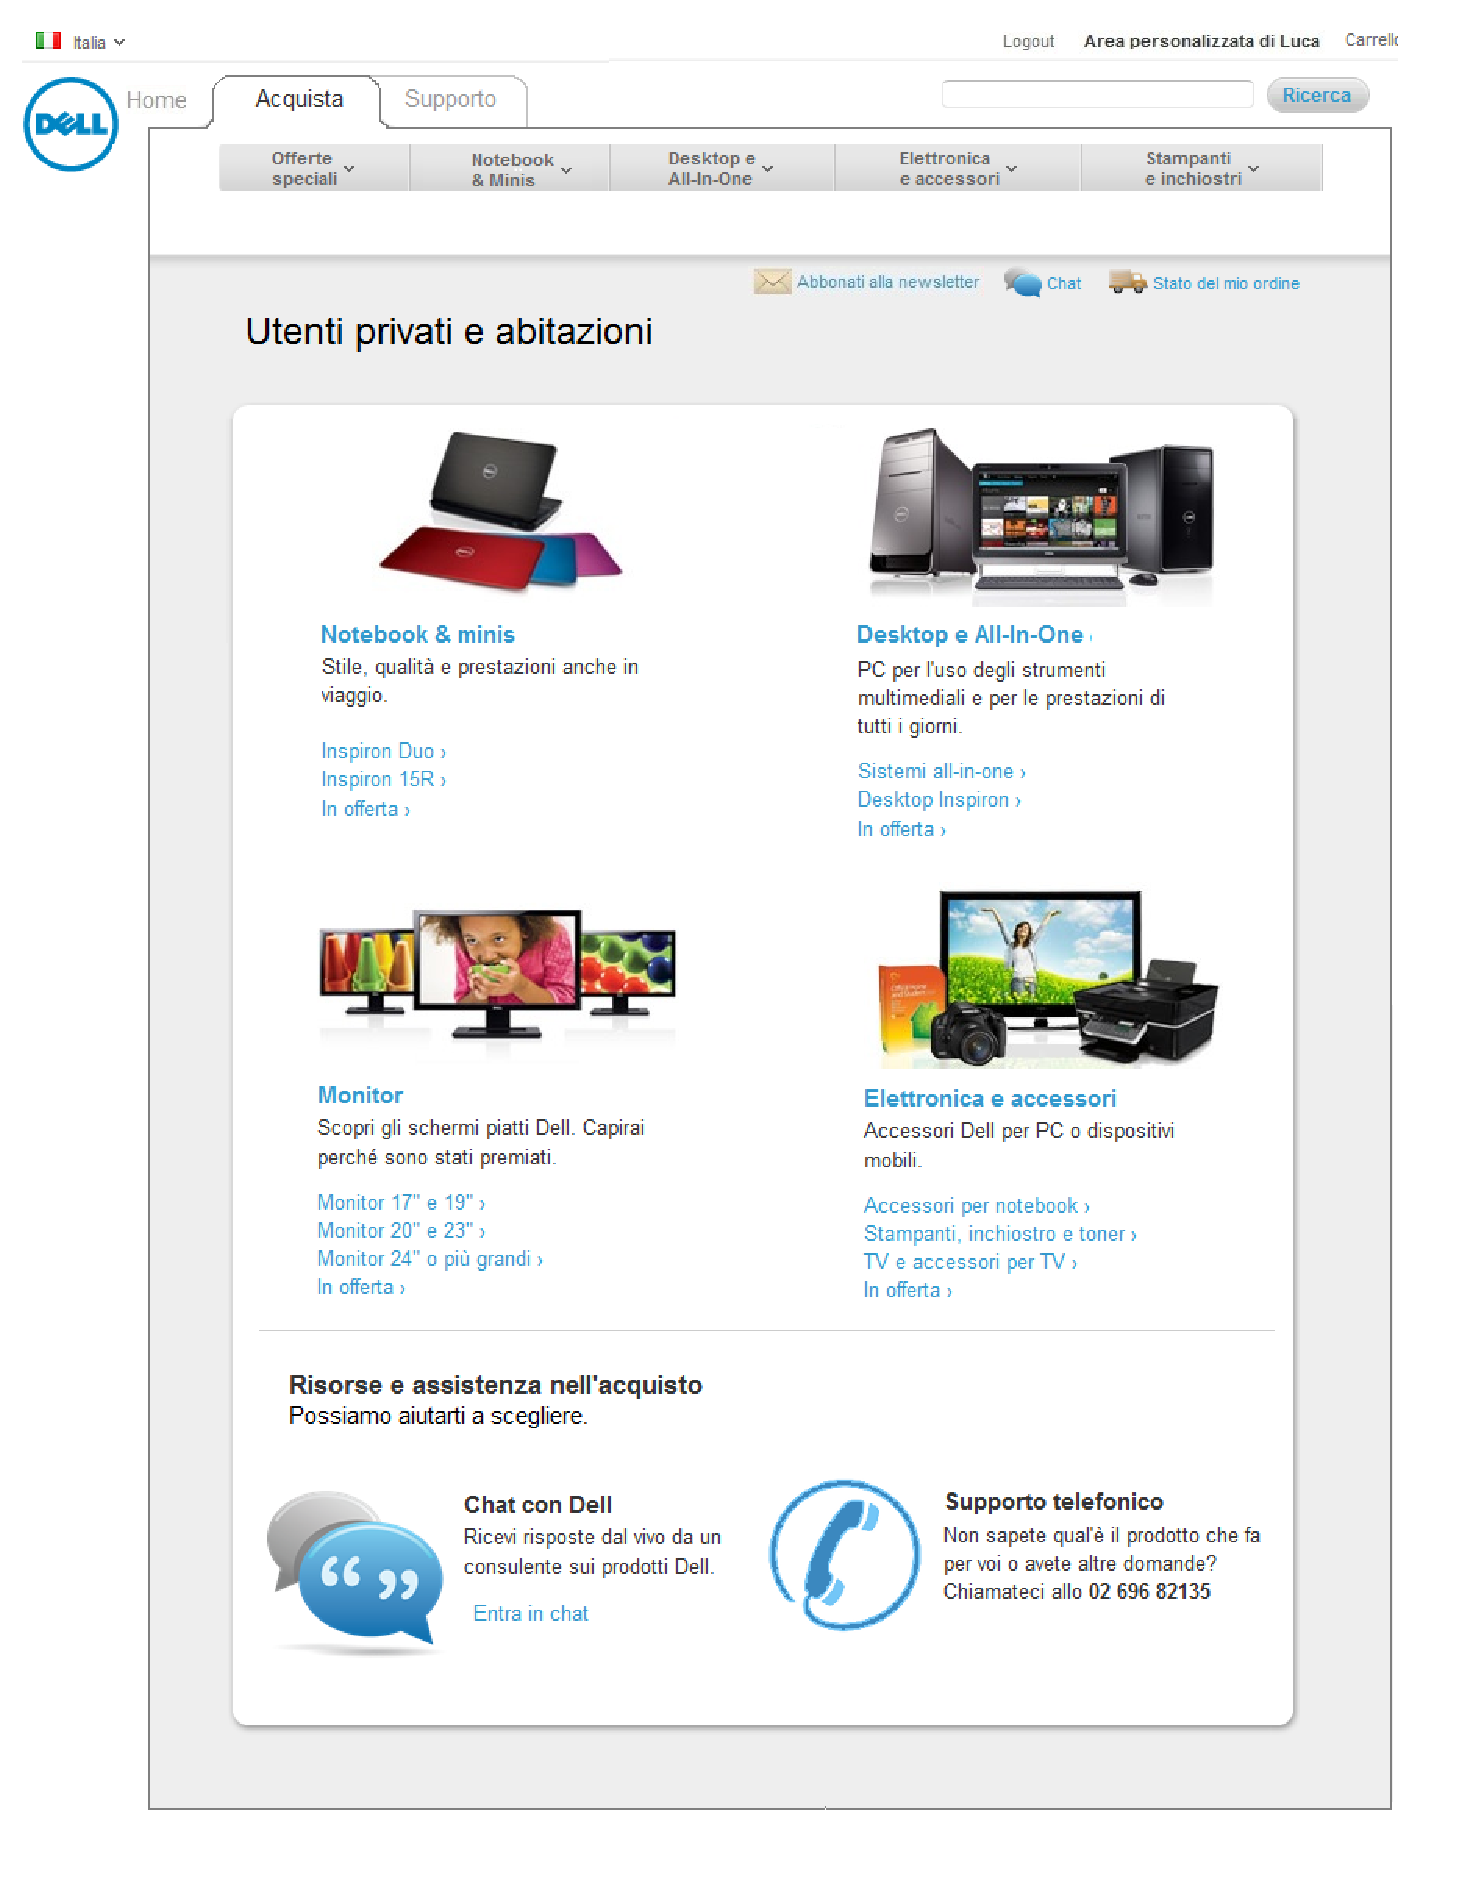
\includegraphics[scale=0.52]{figure/mockup_sez_acquisti_pagina_intera.eps}
\caption{Mock-up della sezione acquisti}
\label{fig:mockup_sez_acquisti_pagina_intera}
\end{figure}

\item{\bf Descrizione}: la sezione di supporto, soffre anch'essa di sovraffollamento di link, spesso ripetuti, che disorientano l'utente meno esperto. In questa sezione non ci sono banner pubblicitari, ma la pagine risultano essere dense di link e testo. Sotto le immagini spesso vengono proposte lunghe liste di link, che rallentano la ricerca dei contenuti desiderati.
{\bf Proposte di soluzione}: per migliorare la pagina sono state introdotte radicali modifiche al layout:
\begin{itemize}
\item I quattro gruppi principali di icone poste a centro pagina, sono stati unite ai sei che si trovano poco pi� sotto, all'interno della parte ``Altri strumenti di supporto''. In tal modo si sono ottenuti sette macro sezioni, che racchiudono e suddividono in categorie le tipologie di problemi che potrebbe avere l'utente. Tali categorie sono:
\begin{itemize}
\item Driver e Hardware: sezione dedicata ai driver, aggiornamenti e richiesta di assistenza per  l'hardware del computer. Da tale sezione di pu� accedere alla sezione di download di aggiornamenti per firmware e altro software strttamente legato al funzionamento dei componenti fisici del computer.
\item Guide e Tutorial: sezione dedicata alla documentazione per poter consentire all'utente di consultare manuali e trovare risposte alla domande pi� frequenti.
\item Supporto per Windows: sezione che riguarda tutti i sistemi Microsoft che sono venduti sulle macchine Dell. All'interno si accede a una pagina che permette all'utente di scegliere fra i vari sistemi operativi, trovare risposte che riguardano il buon funzionamento del sistema operativo.
\item Stato dell'ordine e supporto: sezione rivolta a chi necessita di avere risposte e assistenza per effettuare correttamente un ordine, avere notizie riguardate lo stato si un ordine gi� effettuato.
\item Sicurezza e virus: sezione dedicata alla sicurezza del sistema Dell acquistato.
\item Connettivit� e reti: sezione dedicata alla configurazione e gestione di una rete domestica, sia calbata che wireless.
\item Stampanti e altre periferiche: sezione dedicata all'installazione e configurazione in una periferica collegata poi a un sistema Dell. In tale sezione si trova anche supporto per le periferiche di marchio Dell.
\end{itemize}
\item Sotto alle sette categorie di cui sopra ne abbiamo poste altre quattro che non accorpabili alle  precedenti, e sono meno importanti delle precedenti:
\begin{itemize}
\item Forum Dell: link dedicato all'accesso alla community per avere assistenza da altri utenti.
\item Informazioni sulla garanzia: link che permette di accedere alla visione del contratto di garanzia che l'utente stipula al momento dell'acquisto di un prodotto Dell.
\item Cronologia e stato di supporto: qualora la richiesta di assistenza non fosse immediatamente soddisfatta, in questa sezione l'utente pu� avere informazioni e aggiornamenti sulla propria domanda di supporto.
\item Strumenti e applicazioni: sezione dedicata a come trovare i vari codici, e diciture dei compoenti hardware e software che sono spesso richiesti dall'assistenza.
\end{itemize}
\item A fianco del corpo centrale, a sinistra � riproposta una colonna di link, che a dispetto della versione precedente (figura: \ref{fig:supporto_senza_modifiche}), ha molti meno link. Nella nuova versione infatti sono stati riportati solamente:
\begin{itemize}
\item un link all'home page della sezione di supporto;
\item una serie di contatti diretti con gli operatori specializzati (vendita, ordine, tecnici).
\item una lista composta da otto link, che riportano le otto domande pi� frequenti poste nell'ultimo periodo. Tale lista � variabile, in quanto le domande poste pi� spesso cambieranno nel tempo, abbiamo ritenuto utile mostrarle come acceleratori.
\end{itemize}
\end{itemize}
\end{itemize}
\begin{figure}[t]
\centering
\includegraphics[scale=0.5]{figure/supporto_senza_modifiche.eps}
\caption{Home page della sezione di supporto prima delle modifiche}
\label{fig:supporto_senza_modifiche}
\end{figure}

\begin{figure}[!h]
\centering
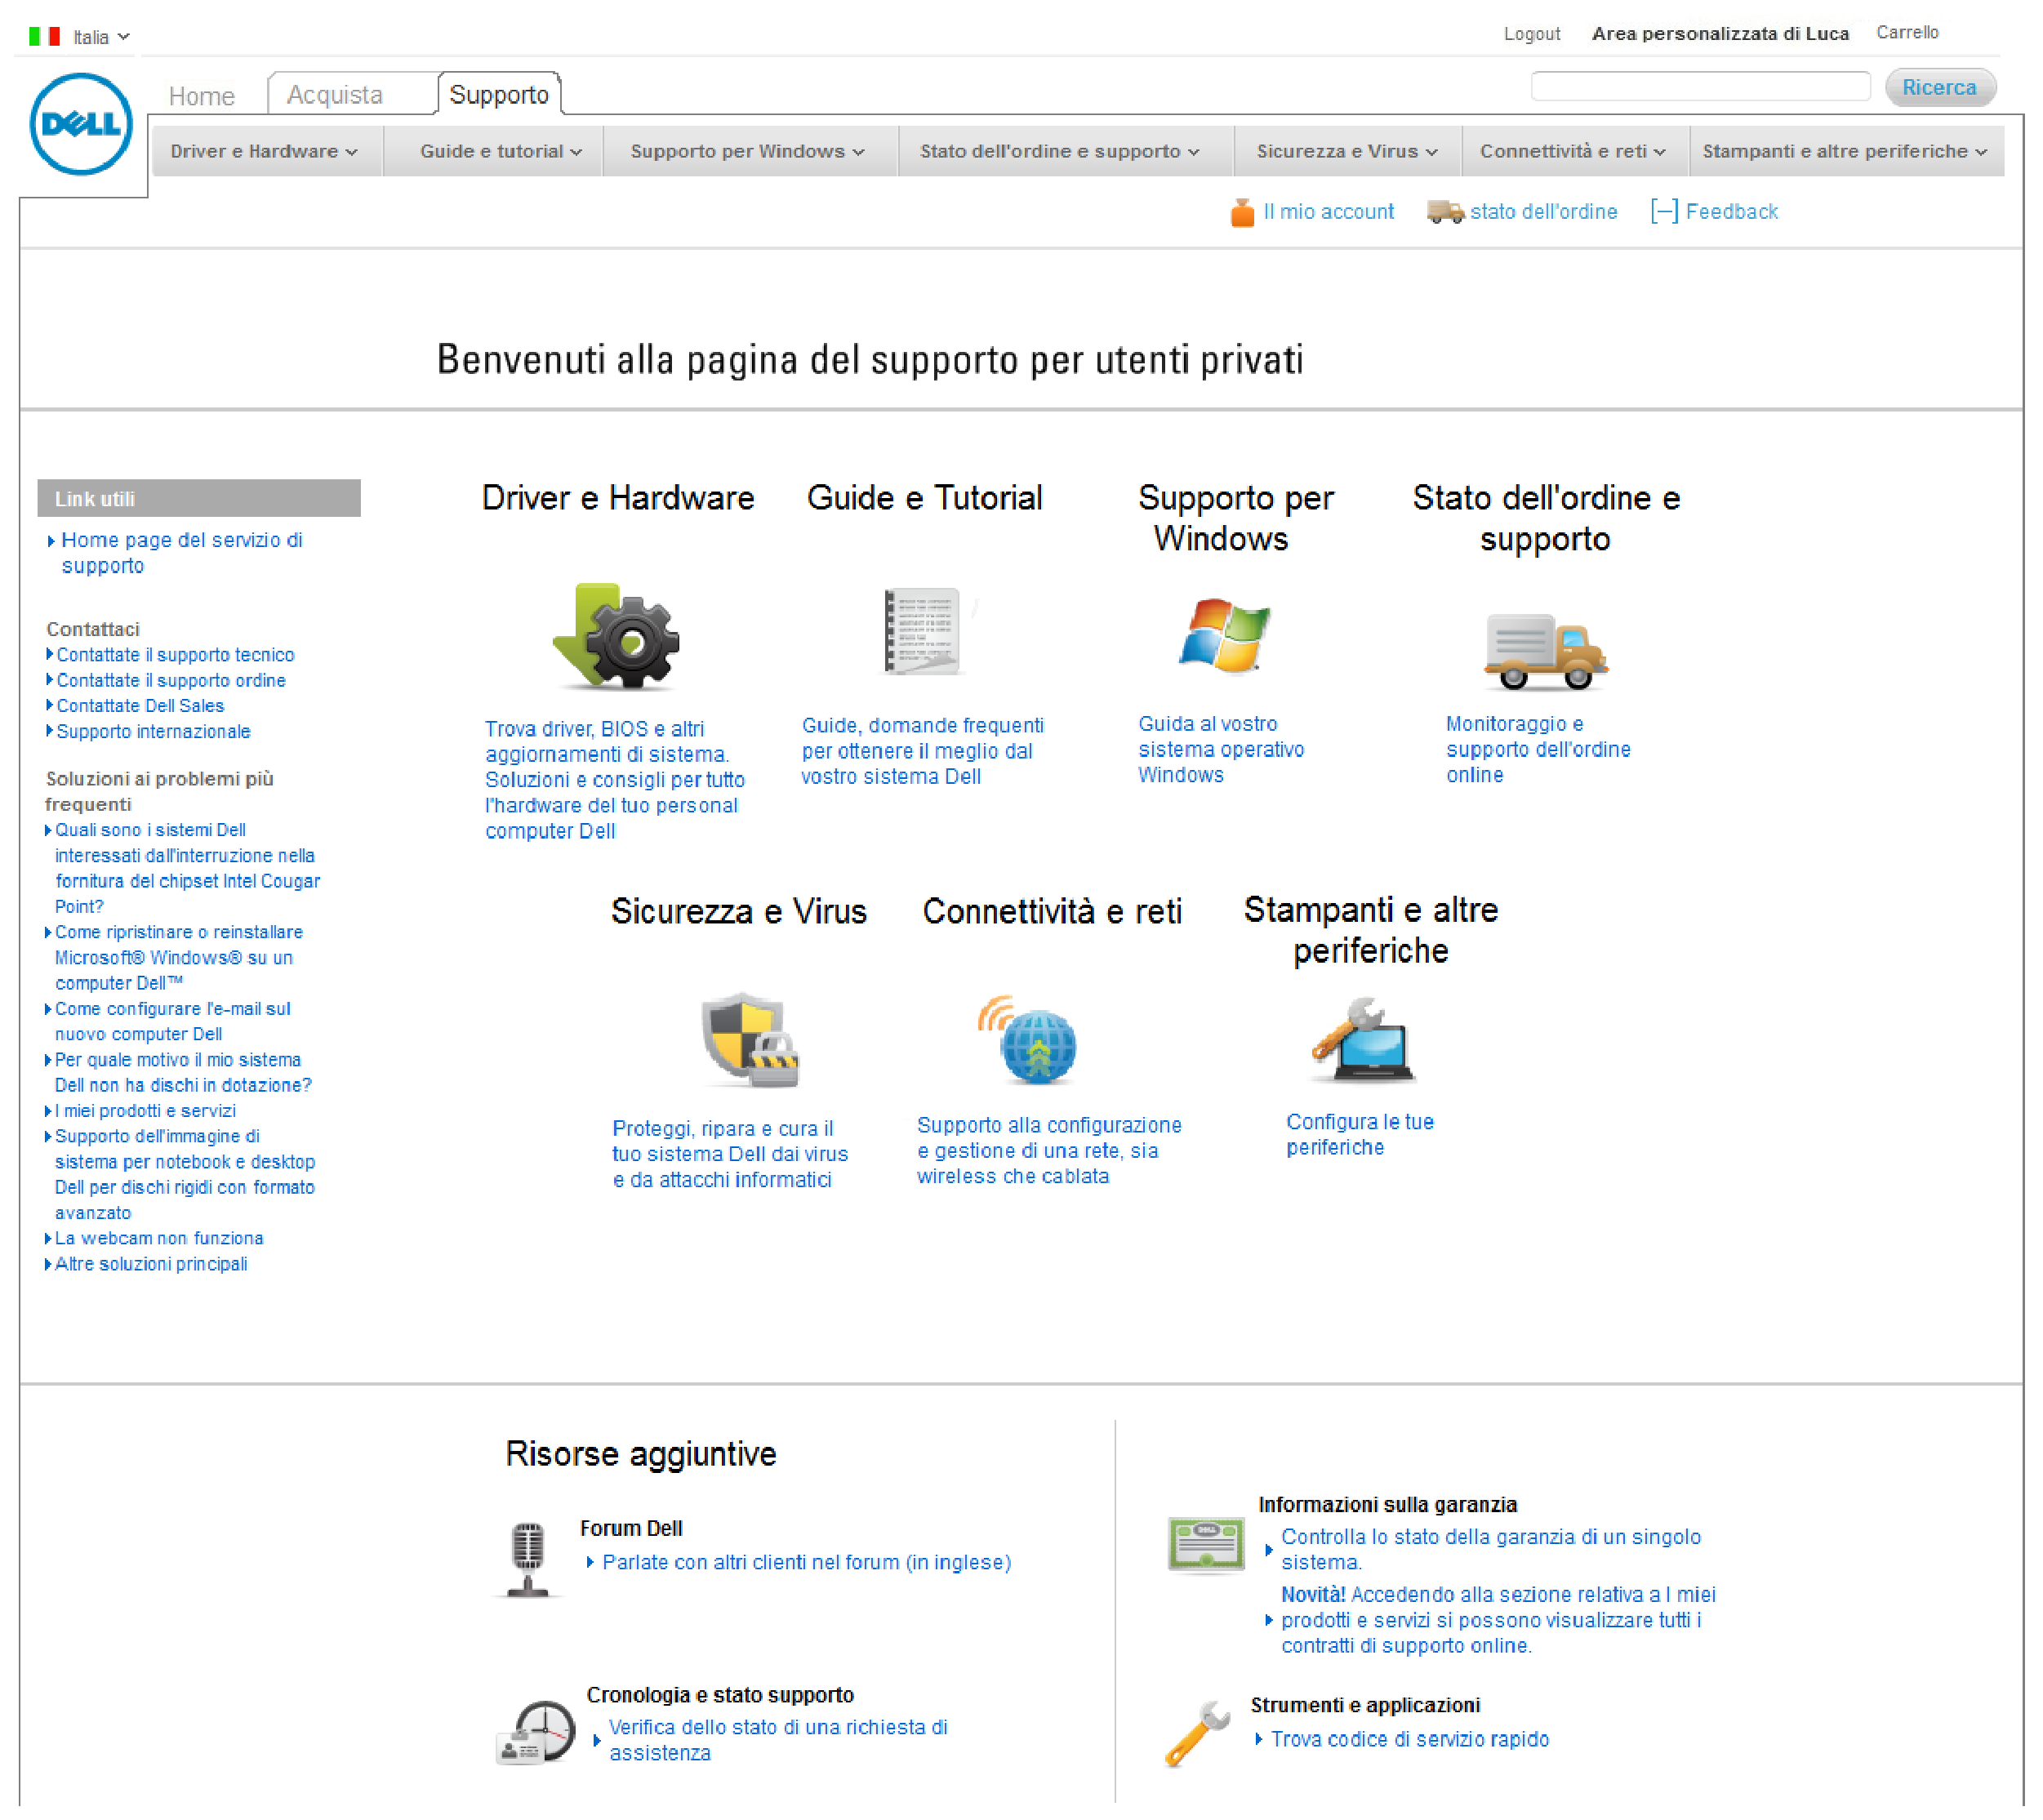
\includegraphics[angle=90,scale=0.45]{figure/mock_up_home_supporto.eps}
\caption{Mock-up della home page della sezione di supporto}
\label{fig:mock_up_home_supporto}
\end{figure}

